\chapter{热学(选修3-3)}
\section{分子动理论 内能}


\begin{longtable}[]{@{}lll@{}}
\toprule
考纲要求 & 考情分析 & 命题趋势\tabularnewline
\midrule
\endhead
\begin{minipage}[t]{0.30\columnwidth}\raggedright
1.微观量的估算Ⅰ

2.分子力、分子势能与分子间距的关系Ⅰ

3.物体的内能Ⅰ\strut
\end{minipage} & \begin{minipage}[t]{0.30\columnwidth}\raggedright
2017·北京卷,13

2017·江苏卷,12

2016·全国卷\uppercase\expandafter{\romannumeral3},33(1)\strut
\end{minipage} & \begin{minipage}[t]{0.30\columnwidth}\raggedright
高考对本部分知识的考查主要以选择题或填空题形式出现,且为选考内容.高考只要求理解物理概念和物理规律的确切含义,理解物理规律的适用条件\strut
\end{minipage}\tabularnewline
\bottomrule
\end{longtable}



1.分子动理论的基本观点和实验依据、阿伏加德罗常数

(1)物体是由大量分子组成的

\ding{172}分子的大小

a.分子的直径(视为球模型):数量级为\_\_10-10\_\_m;

b.分子的质量:数量级为10-26 kg.

\ding{173}阿伏加德罗常数

a.1
mol的任何物质都含有相同的粒子数.通常可取NA=\_\_6.02\ding{54}1023\_\_mol-1;

b.阿伏加德罗常数是联系宏观物理量和微观物理量的桥梁.

(2)分子永不停息地做无规则运动

\ding{172}扩散现象

a.定义:\_\_不同\_\_物质能够彼此进入对方的现象;

b.实质:扩散现象并不是外界作用引起的,也不是化学反应的结果,而是由分子的无规则运动产生的物质迁移现象,温度\_\_越高\_\_,扩散现象越明显.

\ding{173}布朗运动

a.定义:悬浮在液体中的\_\_小颗粒\_\_的永不停息地无规则运动;

b.实质:布朗运动反映了\_\_液体分子\_\_的无规则运动;

c.特点:颗粒越\_\_小\_\_,运动越明显,温度越\_\_高\_\_,运动越剧烈.

\ding{174}热运动

a.分子永不停息地做\_\_无规则\_\_运动叫做热运动;

b.特点:分子的无规则运动和温度有关,温度越高,分子运动越激烈.

(3)分子间同时存在引力和斥力

\ding{172}物质分子间存在空隙,分子间的引力和斥力是\_\_同时\_\_存在的,实际表现出的分子力是引力和斥力的\_\_合力\_\_;

\ding{173}分子力随分子间距离变化的关系:分子间的引力和斥力都随分子间距离的增大而\_\_减小\_\_,随分子间距离的减小而\_\_增大\_\_,但斥力比引力变化得\_\_快\_\_;

\ding{174}分子力与分子间距离的关系图线由分子间的作用力与分子间距离关系图线(如图所示)可知:

\begin{center}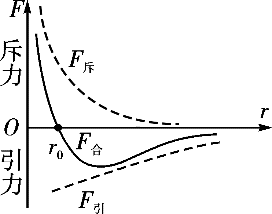
\includegraphics[width=1.23611in,height=0.97153in]{media/image485.png}\end{center}
a.当r=r0时,F引=F斥,分子力为\_\_零\_\_;

b.当r\textgreater r0时,F引\textgreater F斥,分子力表现为\_\_引力\_\_;

c.当r\textless r0时,F引\textless F斥,分子力表现为\_\_斥力\_\_;

d.当分子间距离大于10r0(约为10-9 m)时,分子力很弱,可以忽略不计.

2.温度是分子平均动能的标志 内能

(1)温度

一切达到热平衡的系统都具有相同的\_\_温度\_\_.

(2)两种温标

摄氏温标和热力学温标.关系T=t+273.15 K.

(3)分子的动能

\ding{172}分子动能是\_\_分子热运动\_\_所具有的动能;

\ding{173}分子热运动的平均动能是所有分子热运动的动能的平均值,\_\_温度\_\_是分子热运动的平均动能的标志;

\ding{174}分子热运动的总动能是物体内所有分子热运动动能的\_\_总和\_\_.

(4)分子的势能

\ding{172}意义:由于分子间存在着引力和斥力,所以分子具有由它们的\_\_相对位置\_\_决定的能.

\ding{173}分子势能的决定因素

a.微观上:决定于\_\_分子间距离\_\_和分子排列情况,

b.宏观上:决定于\_\_体积\_\_和状态.

(5)物体的内能

\ding{172}概念理解:物体中所有分子的热运动\_\_动能\_\_与\_\_分子势能\_\_的总和,是状态量;

\ding{173}决定因素:对于给定的物体,其内能大小由物体的\_\_温度\_\_和\_\_体积\_\_决定,即由物体内部状态决定;

\ding{174}影响因素:物体的内能与物体的位置高低、运动速度大小\_\_无关\_\_.

\ding{175}改变物体内能的两种方式:\_\_做功\_\_和\_\_热传递\_\_.

\begin{center}
\includegraphics[width=0.92431in,height=0.21667in]{media/image6.png}\end{center}
1.判断正误

(1)温度越高,扩散现象越明显.( \ding{52} )

(2)布朗运动是液体分子的无规则运动.( \ding{54} )

(3)分子间的引力和斥力都随分子间距的减小而增大.( \ding{52} )

(4)-33 ℃=240 K.( \ding{52} )

(5)物体温度降低,其分子热运动的平均动能增大.( \ding{54} )

(6)当分子力表现为引力时,分子势能随分子间距离的增大而增大.( \ding{52} )

(7)物体温度不变,其内能一定不变.( \ding{54} )

2.钻石是首饰和高强度钻头、刻刀等工具中的主要材料.设钻石的密度为ρ
(kg/m3),摩尔质量为M
(g/mol),阿伏加德罗常数为NA,已知1克拉=0.2克,则( C )

A.a克拉钻石所含有的分子数为

B.a克拉钻石所含有的分子数为

C.每个钻石分子直径的表达式为(单位为m)

D.每个钻石分子直径的表达式为(单位为m)

解析 a克拉钻石物质的量为n=,所含分子数为N=nNA=,选项A、B错误;钻石的摩尔体积为V=(单位为m3/mol),每个钻石分子体积为V0==,设钻石分子直径为d,则V0=π3,联立解得d=(单位为m).选项C正确,D错误.

3.(多选)关于对内能的理解,下列说法正确的是( AD )

A.系统的内能是由系统的状态决定的

B.做功可以改变系统的内能,但是单纯地对系统传热不能改变系统的内能

C.不计分子之间的分子势能,质量和温度相同的氢气和氧气具有相同的内能

D.1 g 100 ℃水的内能小于1 g 100 ℃水蒸气的内能


\begin{center}
\includegraphics[width=0.92431in,height=0.21667in]{media/image11.png}\end{center}
\subsection{微观量的估计}

1.求解分子直径时的两种模型(对于固体和液体)

(1)把分子看成球形,d=.

(2)把分于看成小立方体,d=

提醒:对于气体,利用d=算出的不是分子直径,而是气体分于间的平均距离.

2.宏观量与微观量的相互关系

(1)微观量:分子体积V0、分子直径d、分子质量m0.

(2)宏观量:物体的体积V、摩尔体积Vmol、物体的质量m、摩尔质量M、物体的密度ρ.

(3)相互关系

\ding{172}一个分子的质量:m0==;

\ding{173}一个分子的体积:V0==;(注:对气体V0为分子所占空间体积)

\ding{174}物体所含的分子数:n=NA=NA或n=NA=NA.

\begin{center}
\includegraphics[width=0.70764in,height=0.12292in]{media/image13.png}\end{center}
微观量的求解方法

(1)分子的大小、分子体积、分子质量属微观量,直接测量它们的数值非常困难,可以借助较易测量的宏观量结合摩尔体积、摩尔质量等来估算这些微观量,其中阿伏加德罗常数是联系宏观量和微观量的桥梁和纽带.

(2)建立合适的物理模型,通常把固体、液体分子模拟为球形或小立方体形.气体分子所占据的空间则建立立方体模型.

{[}例1{]}(2018·浙江绍兴质检)空调在制冷过程中,室内空气中的水蒸气接触蒸发器(铜管)液化成水,经排水管排走,空气中水分越来越少,人会感觉干燥.若有一空调工作一段时间后,排出液化水的体积V=1.0\ding{54}103
cm3,已知水的密度ρ=1.0\ding{54}103 kg/m3、摩尔质量M=1.8\ding{54}10-2
kg/mol,阿伏加德罗常数NA=6.0\ding{54}1023 mol-1.试求:(结果均保留一位有效数字)

(1)该液化水中含有水分子的总数N;

(2)一个水分子的直径d.

答案 (1)3\ding{54}1025个 (2)4\ding{54}10-10 m

\subsection{分子热运动与布朗运动}

布朗运动与分子热运动的比较

\begin{longtable}[]{@{}lll@{}}
\toprule
& 布朗运动 & 分子热运动\tabularnewline
\midrule
\endhead
共同点 & 都是无规则运动,都随温度的升高而变得更加剧烈 &\tabularnewline
不同点 & 小颗粒的运动 & 分子的运动\tabularnewline
& 使用光学显微镜观察 & 使用电子显微镜观察\tabularnewline
联系 &
布朗运动是由于小颗粒受到周围分子热运动的撞击力而引起的,反映了分子做无规则运动
&\tabularnewline
\bottomrule
\end{longtable}

{[}例2{]}(2017·江苏卷)(1)甲图和乙图是某同学从资料中查到的两张记录水中炭粒运动位置连线的图片,记录炭粒位置的时间间隔均为30
s,两方格纸每格表示的长度相同.比较两张图片可知:若水温相同,\_\_甲\_\_(选填``甲''或``乙'')中炭粒的颗粒较大;若炭粒大小相同,\_\_乙\_\_(选填``甲''或``乙'')中水分子的热运动较剧烈.

\begin{center}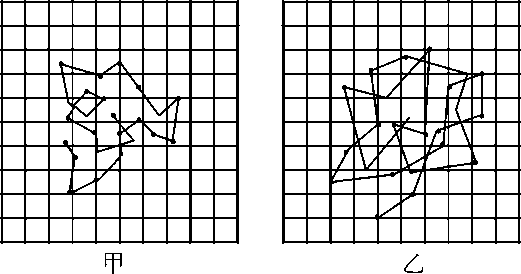
\includegraphics[width=2.36806in,height=1.24514in]{media/image486.png}\end{center}
(2)科学家可以运用无规则运动的规律来研究生物蛋白分子.资料显示,某种蛋白的摩尔质量为66
kg/mol,其分子可视为半径为3\ding{54}10-9 m的球,已知阿伏加德罗常数为6.0\ding{54}1023
mol-1.请估算该蛋白的密度.(计算结果保留一位有效数字)

解析 (1)相同温度和条件下,炭粒较大的其布朗运动的激烈程度较弱,炭粒在30
s始、末时刻所在位置连线的距离就较短,故甲图中炭粒的颗粒较大;炭粒大小相同时,温度越高,分子的热运动越剧烈,做布朗运动的炭粒运动也越剧烈,故乙中水分子的热运动较剧烈.

(2)摩尔体积Vmol=πr3NA{[}或Vmol=(2r)3NA{]},

由密度ρ=,解得ρ=,

代入数据得ρ=1\ding{54}103 kg/m3(或ρ=5\ding{54}102 kg/m3,5\ding{54}102~1\ding{54}103 kg/m3都算对).

答案 (2)见解析

\subsection{分子与分子势能}

对分子势能的理解

分子势能与分子间的距离(宏观表现为物体的体积)有关,分子势能的大小随距离的变化如图所示,由图可知:

\begin{center}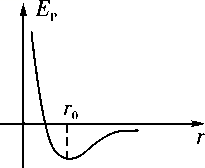
\includegraphics[width=0.93403in,height=0.76389in]{media/image487.png}\end{center}
1.当分子力为零时,即r=r0时,分子势能不是零,而是最小.

2.当r\textgreater r0时,分子力表现为引力,随着分子间距离增大,分子需要不断克服分子力做功,分子势能增大.

3.当r\textless r0时,分子力表现为斥力,随着分子间距离减小,分子需要不断克服分子力做功,分子势能增大.

4.分子势能的数值和其他势能-样,也具有相对意义,由图可知,选无穷远处为零分子势能时,分子势能可以大于零,可以小于零,也可以等于零;但如果选r=r0处为零势能点,则分子势能只能大于零.但是无论选哪个位置为零势能点,在r=r0处分子势能都是最小的.

5.物体体积改变,物体分子势能必定发生改变.

{[}例3{]}(2017·福建福州市模块验收测试)(多选)两分子间的斥力和引力的合力F与分子间距离r的关系如图中曲线所示,曲线与r轴交点的横坐标为r0.相距很远的两分子在分子力作用下,由静止开始相互接近.若两分子相距无穷远时分子势能为零,下列说法正确的是( ACE )

\begin{center}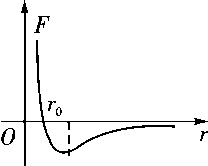
\includegraphics[width=0.94306in,height=0.75486in]{media/image488.png}\end{center}
A.在r\textgreater r0阶段,F做正功,分子动能增加,势能减小

B.在r\textless r0阶段,F做负功,分子动能减小,势能也减小

C.在r=r0时,分子势能最小,动能最大

D.在r=r0时,分子势能为零

E.分子动能和势能之和在整个过程中不变

\begin{center}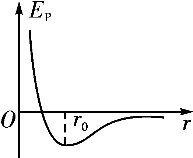
\includegraphics[width=0.87708in,height=0.71667in]{media/image489.png}\end{center}
解析 由Ep-r图可知:在r\textgreater r0阶段,当r减小时F做正功,分子势能减小,分子动能增加,故选项A正确;在r\textless r0阶段,当r减小时F做负功,分子势能增加,分子动能减小,故选项B错误;在r=r0时,分子势能最小,但不为零,动能最大,故选项C正确,D错误;在整个相互接近的过程中,分子动能和势能之和保持不变,故选项E正确.

\section{固体、液体和气体}

1.晶体和非晶体

\begin{longtable}[]{@{}llll@{}}
\toprule
分类比较   & 晶体 & 非晶体 &\tabularnewline
\midrule
\endhead
& 单晶体 & 多晶体 &\tabularnewline
外形 & 规则 & \_\_不规则\_\_ & 不规则\tabularnewline
熔点 & 确定 & 不确定 &\tabularnewline
物理性质 & 各向\_\_异性\_\_ & 各向\_\_同性\_\_ &\tabularnewline
原子排列 & \_\_有规则\_\_,但多晶体每个单晶体间的排列无规则 & 无规则
&\tabularnewline
形成与转化 &
有的物质在不同条件下能够形成不同的\_\_晶体\_\_.同一物质可能以\_\_晶体\_\_和非晶体两种不同的形态出现,有些晶体在一定条件下也可以转化为\_\_非晶体\_\_.
& &\tabularnewline
典型物质 & 石英、云母、食盐,硫酸铜 & 玻璃、蜂蜡、松香 &\tabularnewline
\bottomrule
\end{longtable}

2 .液体的表面张力 液晶的微观结构

(1)液体的表面张力

\ding{172}作用:液体的\_\_表面张力\_\_使液面具有收缩到表面积最小的趋势;

\ding{173}方向:表面张力跟液面\_\_相切\_\_,且跟这部分液面的分界线\_\_垂直\_\_.

(2)液晶

\ding{172}液晶分子既保持排列有序而显示各向\_\_异性\_\_,又可以自由移动位置,保持了液体的\_\_流动性\_\_;

\ding{173}液晶分子的位置无序使它像\_\_液体\_\_,排列有序使它像\_\_晶体\_\_;

\ding{174}液晶分子的排列从某个方向看比较整齐,而从另外一个方向看则是\_\_杂乱无章\_\_的.

3.气体、气体实验定律和理想气体

(1)气体分子运动的特点

\ding{172}气体分子间距较\_\_大\_\_,分子力可以\_\_忽略\_\_,因此分子间除碰撞外不受其他力的作用,故气体能充满整个空间;

\ding{173}分子做无规则的运动,速率有大有小,且时时变化,大量分子的速率按\_\_``中间多,两头少''\_\_的规律分布;

\ding{174}温度升高时,速率小的分子数\_\_减少\_\_,速率大的分子数\_\_增多\_\_,分子的平均速率将\_\_增大\_\_,但速率分布规律\_\_不变\_\_.

(2)气体的状态参量

\_\_压强\_\_、\_\_体积\_\_、\_\_温度\_\_.

(3)气体的压强

\ding{172}产生原因:由于气体分子无规则的热运动,大量的分子频繁地碰撞器壁产生持续而稳定的\_\_压力\_\_;

\ding{173}大小:气体的压强在数值上等于气体作用在\_\_单位面积\_\_上的压力.公式p=;

\ding{174}决定因素

a.宏观上:决定于气体的温度和体积;

b.微观上:决定于分子的平均动能和分子数密度.

(4)气体实验定律

\begin{longtable}[]{@{}llll@{}}
\toprule
& 玻意耳定律 & 查理定律 & 盖---吕萨克定律\tabularnewline
\midrule
\endhead
\begin{minipage}[t]{0.22\columnwidth}\raggedright
内

容\strut
\end{minipage} & \begin{minipage}[t]{0.22\columnwidth}\raggedright
一定质量的某种气体,在温度不变的情况下,压强与体积成反比\strut
\end{minipage} & \begin{minipage}[t]{0.22\columnwidth}\raggedright
一定质量的某种气体,在体积不变的情况下,压强与热力学温度成正比\strut
\end{minipage} & \begin{minipage}[t]{0.22\columnwidth}\raggedright
一定质量的某种气体,在压强不变的情况下,体积与热力学温度成正比\strut
\end{minipage}\tabularnewline
\begin{minipage}[t]{0.22\columnwidth}\raggedright
表

达

式\strut
\end{minipage} & \begin{minipage}[t]{0.22\columnwidth}\raggedright
\_\_p1V1=p2V2\_\_\strut
\end{minipage} & \begin{minipage}[t]{0.22\columnwidth}\raggedright
!!! = \#\#\#或

!!! = \#\#\#\strut
\end{minipage} & \begin{minipage}[t]{0.22\columnwidth}\raggedright
!!! = \#\#\#或

!!! = \#\#\#\strut
\end{minipage}\tabularnewline
\bottomrule
\end{longtable}

(5)理想气体状态方程

\ding{172}理想气体:在任何温度、任何压强下都遵从气体实验定律的气体;

\ding{173}一定质量的理想气体状态方程:!!! = \#\#\#或!!! =C \#\#\#(C为常量).

4.饱和汽 未饱和汽和饱和汽压 相对湿度

(1)饱和汽与未饱和汽

\ding{172}饱和汽:与液体处于\_\_动态平衡\_\_的蒸汽;

\ding{173}未饱和汽:没有达到\_\_饱和状态\_\_的蒸汽.

(2)饱和汽压

\ding{172}定义:饱和汽所具有的\_\_压强\_\_;

\ding{173}特点:饱和汽压随温度而变.温度越高,饱和汽压\_\_越大\_\_,且饱和汽压与饱和汽的体积\_\_无关\_\_.

(3)湿度

\ding{172}定义:空气的潮湿程度;

\ding{173}绝对湿度:空气中所含\_\_水蒸气\_\_的压强:

\ding{174}相对湿度:在某一温度下,空气中水蒸气的\_\_压强\_\_与同一温度下水的饱和汽压之比,称为空气的相对湿度,即相对湿度(B)=()()\ding{54}100\%
\subsection{固体和液体的性质}

对液体性质的三点说明

(1)液体表面层、附着层的分子结构特点是导致表面张力、浸润和不浸润现象、毛细现象等现象的根本原因.

(2)同一种液体,对一些固体是浸润的,对另一些固体可能不浸润.

(3)液体沸腾的条件是饱和汽压和外部压强相等.

{[}例1{]}(多选)下列说法正确的是( BCD )

A.将一块晶体敲碎后,得到的小颗粒是非晶体

B.固体可以分为晶体和非晶体两类,有些晶体在不同方向上有不同的光学性质

C.由同种元素构成的固体,可能会由于原子的排列方式不同而成为不同的晶体

D.在合适的条件下,某些晶体可以转变为非晶体,某些非晶体也可以转变为晶体

E.在熔化过程中,晶体要吸收热量,但温度保持不变,内能也保持不变

\subsection{气体压强的计算}

平衡状态下气体压强的求法

(1)参考液片法:选取假想的液体薄片(自身重力不计)为研究对象,分析液片两侧受力情况,建立平衡方程,消去面积,得到液片两侧压强相等方程,求得气体的压强.

(2)力平衡法:选与气体接触的液柱(或活塞)为研究对象进行受力分析,得到液柱(或活塞)的受力平衡方程,求得气体的压强.

(3)等压面法:在连通器中,同一种液体(中间不间断)同一深度处压强相等.

{[}例2{]}如图所示,竖直放置的U形管,左端开口,右端封闭,管内有a、b两段水银柱,将A、B两段空气柱封闭在管内.已知水银柱a长10
cm,水银柱b两个液面间的高度差为5 cm,大气压强为75
cmHg,求空气柱A、B的压强.

\begin{center}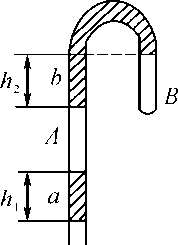
\includegraphics[width=0.81111in,height=1.11319in]{media/image494.png}\end{center}
答案 65 cmHg 60 cmHg

\subsection{气体实验定律及状态方程的应用}

气体实验定律的比较

\begin{longtable}[]{@{}llll@{}}
\toprule
\begin{minipage}[b]{0.22\columnwidth}\raggedright
定律名称比较项目\strut
\end{minipage} & \begin{minipage}[b]{0.22\columnwidth}\raggedright
玻意耳定律

(等温变化)\strut
\end{minipage} & \begin{minipage}[b]{0.22\columnwidth}\raggedright
查理定律

(等容变化)\strut
\end{minipage} & \begin{minipage}[b]{0.22\columnwidth}\raggedright
盖-吕萨克定

律(等压变化)\strut
\end{minipage}\tabularnewline
\midrule
\endhead
\begin{minipage}[t]{0.22\columnwidth}\raggedright
数学

表达式\strut
\end{minipage} & \begin{minipage}[t]{0.22\columnwidth}\raggedright
p1V1=p2V2或

pV=C(常数)\strut
\end{minipage} & \begin{minipage}[t]{0.22\columnwidth}\raggedright
=或

=C(常数)\strut
\end{minipage} & \begin{minipage}[t]{0.22\columnwidth}\raggedright
=或

=C(常数)\strut
\end{minipage}\tabularnewline
\begin{minipage}[t]{0.22\columnwidth}\raggedright
同一气体

的两条

图线\strut
\end{minipage} & \begin{minipage}[t]{0.22\columnwidth}\raggedright
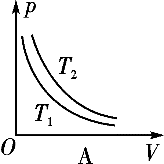
\includegraphics[width=0.74514in,height=0.74514in]{media/image495.png}
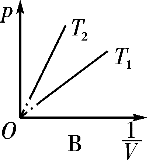
\includegraphics[width=0.70764in,height=0.74514in]{media/image496.png}\strut
\end{minipage} & \begin{minipage}[t]{0.22\columnwidth}\raggedright
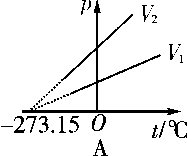
\includegraphics[width=0.84931in,height=0.70764in]{media/image497.png}
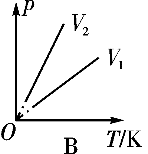
\includegraphics[width=0.67014in,height=0.69792in]{media/image498.png}\strut
\end{minipage} & \begin{minipage}[t]{0.22\columnwidth}\raggedright
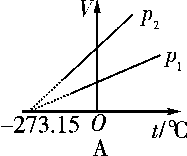
\includegraphics[width=0.84931in,height=0.70764in]{media/image499.png}
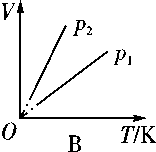
\includegraphics[width=0.70764in,height=0.68889in]{media/image500.png}\strut
\end{minipage}\tabularnewline
\bottomrule
\end{longtable}

{[}例3{]}如图,一固定的竖直气缸由一大一小两个同轴圆筒组成,两圆筒中各有一个活塞.已知大活塞的质量为m1=2.50
kg,横截面积为S1=80.0 cm2;小活塞的质量为m2=1.50
kg,横截面积为S2=40.0 cm2;两活塞用刚性轻杆连接,间距保持为l=40.0
cm;汽缸外大气的压强为p=1.00\ding{54}105 Pa,温度为T=303
K.初始时大活塞与大圆筒底部相距,两活塞间封闭气体的温度为T1=495
K.现汽缸内气体温度缓慢下降,活塞缓慢下移.忽略两活塞与汽缸壁之间的摩擦,重力加速度大小g取10
$10m/s^2$.求:

\begin{center}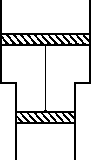
\includegraphics[width=0.41528in,height=0.72639in]{media/image501.png}\end{center}
(1)在大活塞与大圆筒底部接触前的瞬间,缸内封闭气体的温度;

(2)缸内封闭的气体与缸外大气达到热平衡时,缸内封闭气体的压强.

{[}思维导引{]} \ding{172}两气缸活塞面积不等,如何选择受力分析的研究对象?气缸平衡时受到哪几个力作用?\ding{173}第一次下降过程中气体温度下降,气体进行了哪种状态变化?\ding{174}内外气温达到相等过程中气体进行了哪种状态变化?

答案 (1)330 K (2)1.01\ding{54}105 Pa
\section{热力学定律与能量守恒}


1.热力学第一定律

\ding{172}内容:一个热力学系统的\_\_内能增量\_\_等于外界向它传递的热量与外界对它所做的功的和.

\ding{173}表达式:$\Delta$U\_\_Q+W\_\_.

\ding{174}符号法则

\begin{longtable}[]{@{}llll@{}}
\toprule
符号 & W & Q & $\Delta$U\tabularnewline
\midrule
\endhead
+ & 外界对物体做功 & 物体\_\_吸收\_\_热量 &
内能\_\_增加\_\_\tabularnewline
- & 物体对外界做功 & 物体\_\_放出\_\_热量 &
内能\_\_减小\_\_\tabularnewline
\bottomrule
\end{longtable}

2.热力学第二定律的三种表述

(1)克劳修斯表述:热量不能\_\_自发地\_\_从低温物体传到高温物体.

(2)开尔文表述:不可能从\_\_单一\_\_热库吸收热量,使之完全变成功,而\_\_不产生\_\_其他影响.或表述为``第二类永动机不可能制成''.

(3)用熵的概念进行表述:在任何自然过程中,一个孤立系统的总熵不会\_\_减小\_\_(热力学第二定律又叫做熵增加原理).

3.能量守恒定律

(1)内容

能量既不会凭空产生,也不会凭空消失,它只能从一种形式\_\_转化\_\_为另一种形式,或者从一个物体\_\_转移\_\_到别的物体,在转化或转移的过程中,能量的\_\_总和\_\_保持不变.

(2)能源的利用

\ding{172}存在能量耗散和\_\_品质降低\_\_.

\ding{173}重视利用能源时对\_\_环境\_\_的影响.

\ding{174}推进开发新能源,如\_\_太阳能\_\_、生物能、风能、潮汐能等.
\subsection{热力学第一定律}

1.改变内能的两种方式的比较

\begin{longtable}[]{@{}llll@{}}
\toprule
\begin{minipage}[b]{0.22\columnwidth}\raggedright
   方式名称

比较项目   \strut
\end{minipage} & \begin{minipage}[b]{0.22\columnwidth}\raggedright
做功\strut
\end{minipage} & \begin{minipage}[b]{0.22\columnwidth}\raggedright
热传递\strut
\end{minipage} & \begin{minipage}[b]{0.22\columnwidth}\raggedright
\strut
\end{minipage}\tabularnewline
\midrule
\endhead
\begin{minipage}[t]{0.22\columnwidth}\raggedright
区

别\strut
\end{minipage} & \begin{minipage}[t]{0.22\columnwidth}\raggedright
内能变化情况\strut
\end{minipage} & \begin{minipage}[t]{0.22\columnwidth}\raggedright
外界对物体做功,物体的内能增加;物体对外界做功,物体的内能减少\strut
\end{minipage} & \begin{minipage}[t]{0.22\columnwidth}\raggedright
物体吸收热量,内能增加;物体放出热量,内能减少\strut
\end{minipage}\tabularnewline
& 从运动形式上看 & 做功是宏观的机械运动向物体的微观分子热运动的转化 &
热传递则是通过分子之间的相互作用,使同一物体的不同部分或不同物体间的分子热运动发生变化,是内能的转移\tabularnewline
& 从能量的角度看 & 做功是其他形式的能与内能相互转化的过程 &
不同物体间或同一物体不同部分之间内能的转移\tabularnewline
& 能的性质变化情况 & 能的性质发生了变化 & 能的性质不变\tabularnewline
相互联系 & 做一定量的功或传递一定量的热量在改变内能的效果上是相同的 &
&\tabularnewline
\bottomrule
\end{longtable}

2.热力学第一定律不仅反映了做功和热传递这两种改变内能的过程是等效的,而且给出了内能的变化量和做功与热传递之间的定量关系.此定律是标量式,应用时功、内能、热量的单位应统一为国际单位焦耳.

3.三种特殊情况

(1)若过程是绝热的,则$Q=0,W\neq U$,外界对物体做的功等于物体内能的增加;

(2)若过程中不做功,即$W=0,则Q\neq U$,物体吸收的热量等于物体内能的增加;

(3)若过程的始、末状态物体的内能不变,即$\Delta$U=0,则W+Q=0或W=-Q,外界对物体做的功等于物体放出的热量.

\begin{center}
\includegraphics[width=0.70764in,height=0.12292in]{media/image34.png}\end{center}
理想气体内能变化的判定

对一定质量的理想气体,由于无分子势能,其内能只包含分子无规则热运动的动能,这时内能只与温度有关,故判定一定质量的理想气体内能是否变化,应看温度是否发生了变化,与体积无关.

{[}例1{]}(2017·全国卷\uppercase\expandafter{\romannumeral3})如图,一定质量的理想气体从状态a出发,经过等容过程ab到达状态b,再经过等温过程bc到达状态c,最后经等压过程ca回到初态a.下列说法正确的是\_\_ABD\_\_.(选填正确答案标号.选对1个得2分,选对2个得4分,选对3个得5分.每选错1个扣3分,最低得分为0分)

\begin{center}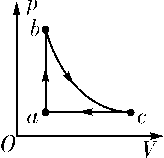
\includegraphics[width=0.74514in,height=0.71667in]{media/image506.png}\end{center}
A.在过程ab中气体的内能增加

B.在过程ca中外界对气体做功

C.在过程ab中气体对外界做功

D.在过程bc中气体从外界吸收热量

E.在过程ca中气体从外界吸收热量

\subsection{热力学第二定律}

1.热力学过程方向性实例

(1)高温物体低温物体

(2)功热量

(3)气体体积V1气体体积V2(较大)

(4)不同气体A和B混合气体AB

2.热力学第一定律和热力学第二定律的关系

热力学第一定律是和热现象有关的物理过程中能量守恒的特殊表达形式及热量与内能改变的定量关系.而第二定律指明了能量转化与守恒能否实现的条件和过程进行的方向,指出了一切变化过程的自然发展是不可逆的,除非靠外界影响.所以二者相互联系,又相互补充.

3.两类永动机的比较

\begin{longtable}[]{@{}ll@{}}
\toprule
第一类永动机 & 第二类永动机\tabularnewline
\midrule
\endhead
不消耗能量却可以源源不断地对外做功的机器 &
从单一热源吸热,全部用来对外做功而不引起其他变化的机器\tabularnewline
违背能量守恒,不可能实现 &
不违背能量守恒,违背热力学第二定律,不可能实现\tabularnewline
\bottomrule
\end{longtable}

{[}例2{]}(2017·江苏模块验收测试)如图所示为电冰箱的工作原理示意图.压缩机工作时,强迫制冷剂在冰箱内外的管道中不断循环.在蒸发器中制冷剂汽化吸收箱体内的热量,经过冷凝器时制冷剂液化,放出热量到箱体外.

\begin{center}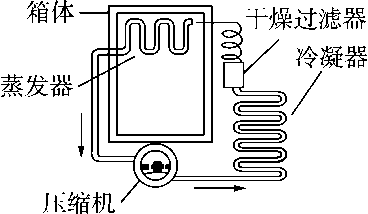
\includegraphics[width=1.67014in,height=0.97153in]{media/image507.png}\end{center}
(1)(多选)下列说法正确的是!!! BC \#\#\#.

A.热量可以自发地从冰箱内传到冰箱外

B.电冰箱的制冷系统能够不断地把冰箱内的热量传到外界,是因为其消耗了电能

C.电冰箱的工作原理不违反热力学第一定律

D.电冰箱的工作原理违反热力学第一定律

(2)电冰箱的制冷系统从冰箱内吸收的热量与释放到外界的热量相比,有怎样的关系?

答案 (2)见解析

\begin{center}
\includegraphics[width=0.70764in,height=0.12292in]{media/image13.png}\end{center}
热力学第二定律的涵义

(1)``自发地''指明了热传递等热力学宏观现象的方向性,不需要借助外界提供能量的帮助.

(2)``不产生其他影响''的含义是发生的热力学宏观过程只在本系统内完成,对周围环境不产生热力学方面的影响,如吸热、放热、做功等.
